% Start a document. In this exaple, we are building an article for a4 paper and 11pt text size. 
\documentclass[11pt,a4paper]{article}

% The preamble is used to import packeges and define variables. 
% There are plenty of options for the preample. Check the manual at https://en.wikibooks.org/wiki/LaTeX
% The easiest way to ensure that you have all the needed packages for any LaTeX project is to download e.g. 
% the MiKTeX distribution (Windows), MacTeX (OS X) 

%Encode input
\usepackage[latin1]{inputenc}

%select language English by using the bable package and use additional packages for math, images etc. 
\usepackage[english]{babel}
\usepackage{amsmath}
\usepackage{amsfonts}
\usepackage{amssymb}
\usepackage{graphicx}
\usepackage{grffile}
\usepackage[left=2cm,right=2cm,top=2cm,bottom=2cm]{geometry}

% TikZ (TikZ ist kein Zeichnenprogramm) is a language to produce vector graphics. 
\usepackage{tikz}

% Some calculations and plottimgs can be made directely in TeX. See the TikZ exemple
\usetikzlibrary{calc}

% The verbatim package lets you imput text that is not interpreted by the compilor. 
\usepackage{verbatim}




% After the begin command, the actual document is created
\begin{document}


This document is written in \LaTeX.

Here is a plot generated in matplotlib from the script result1.py:

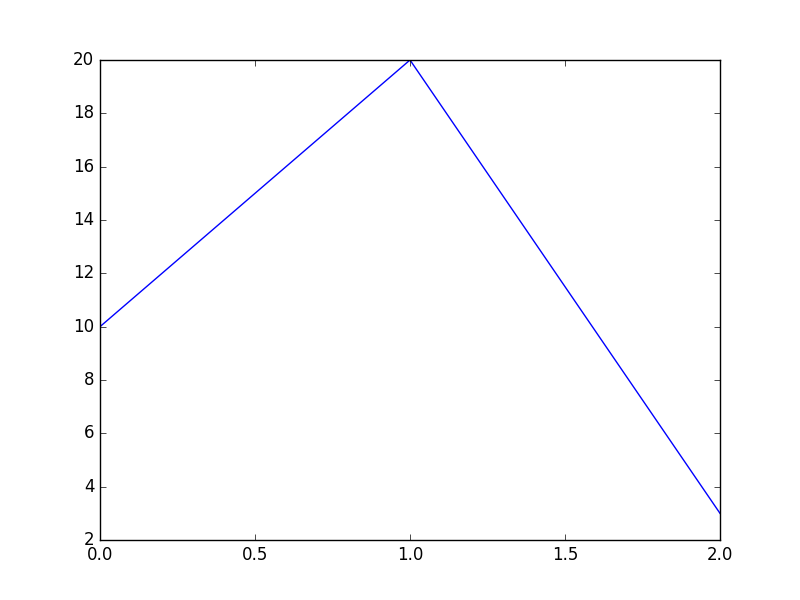
\includegraphics[scale=0.5]{fig/plot1.png}

Here is a more complex plot, also generated from matplotlib. 

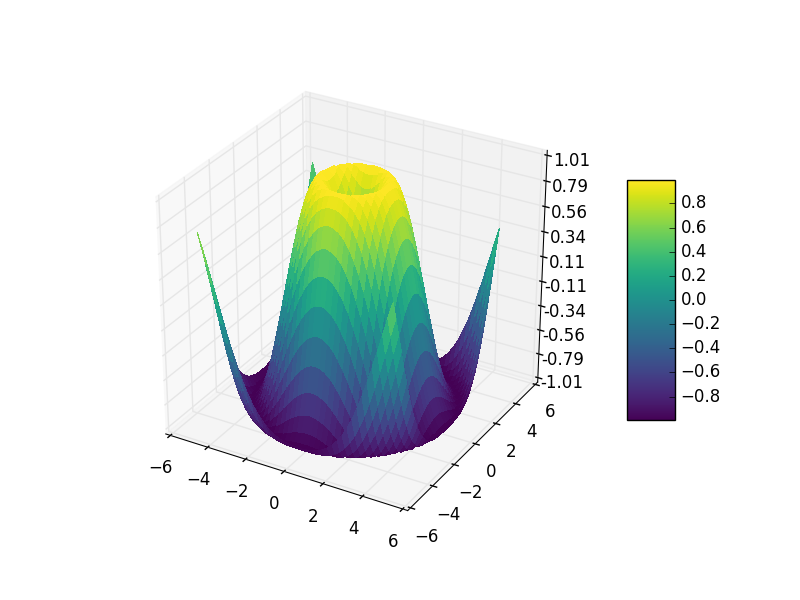
\includegraphics[scale=0.5]{fig/plot2.png}


Here is some more text, imported from a textfile generated by a python script. 

\input{txt/results1.txt}

An here is a map generated by a shellscript

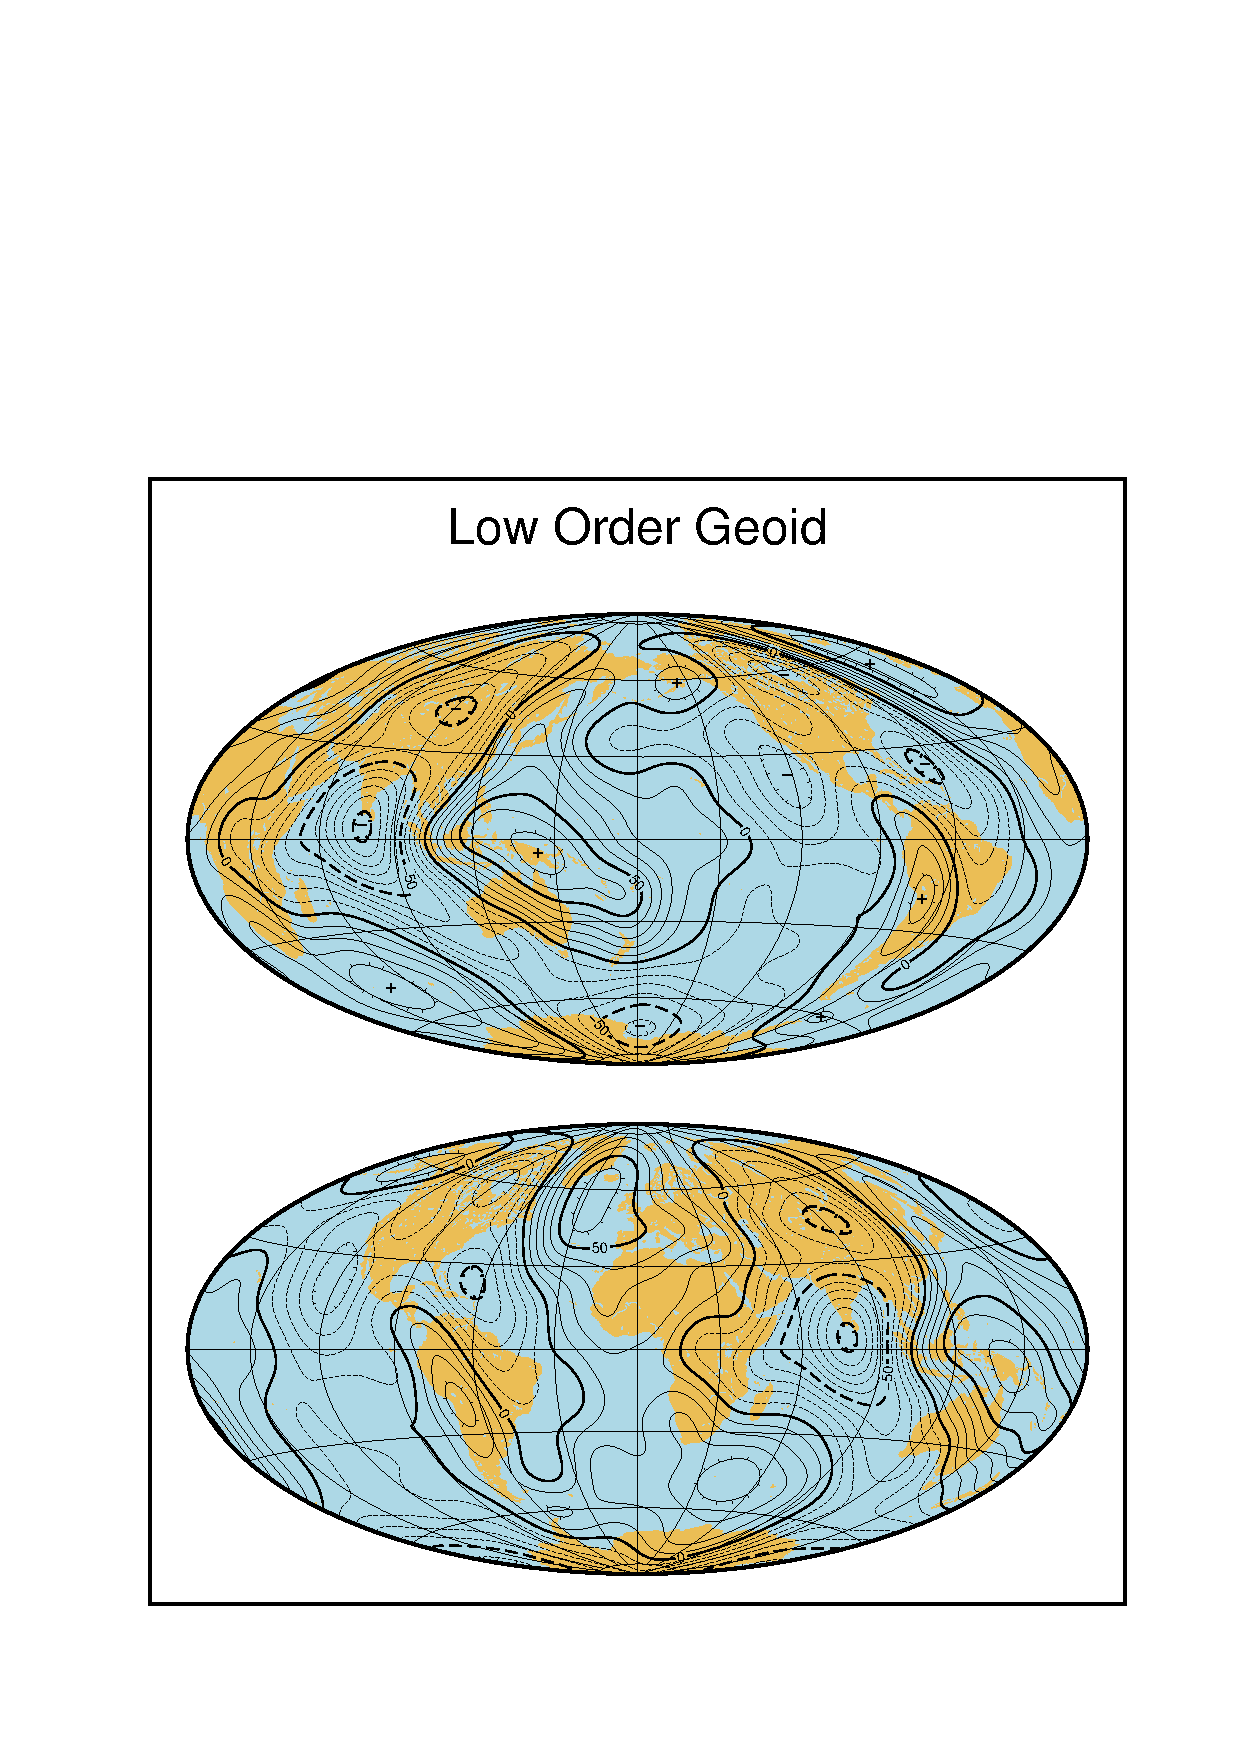
\includegraphics[scale=0.5]{fig/map1.pdf}


\includegraphics[scale=0.5]{img/graptolite.jpg}
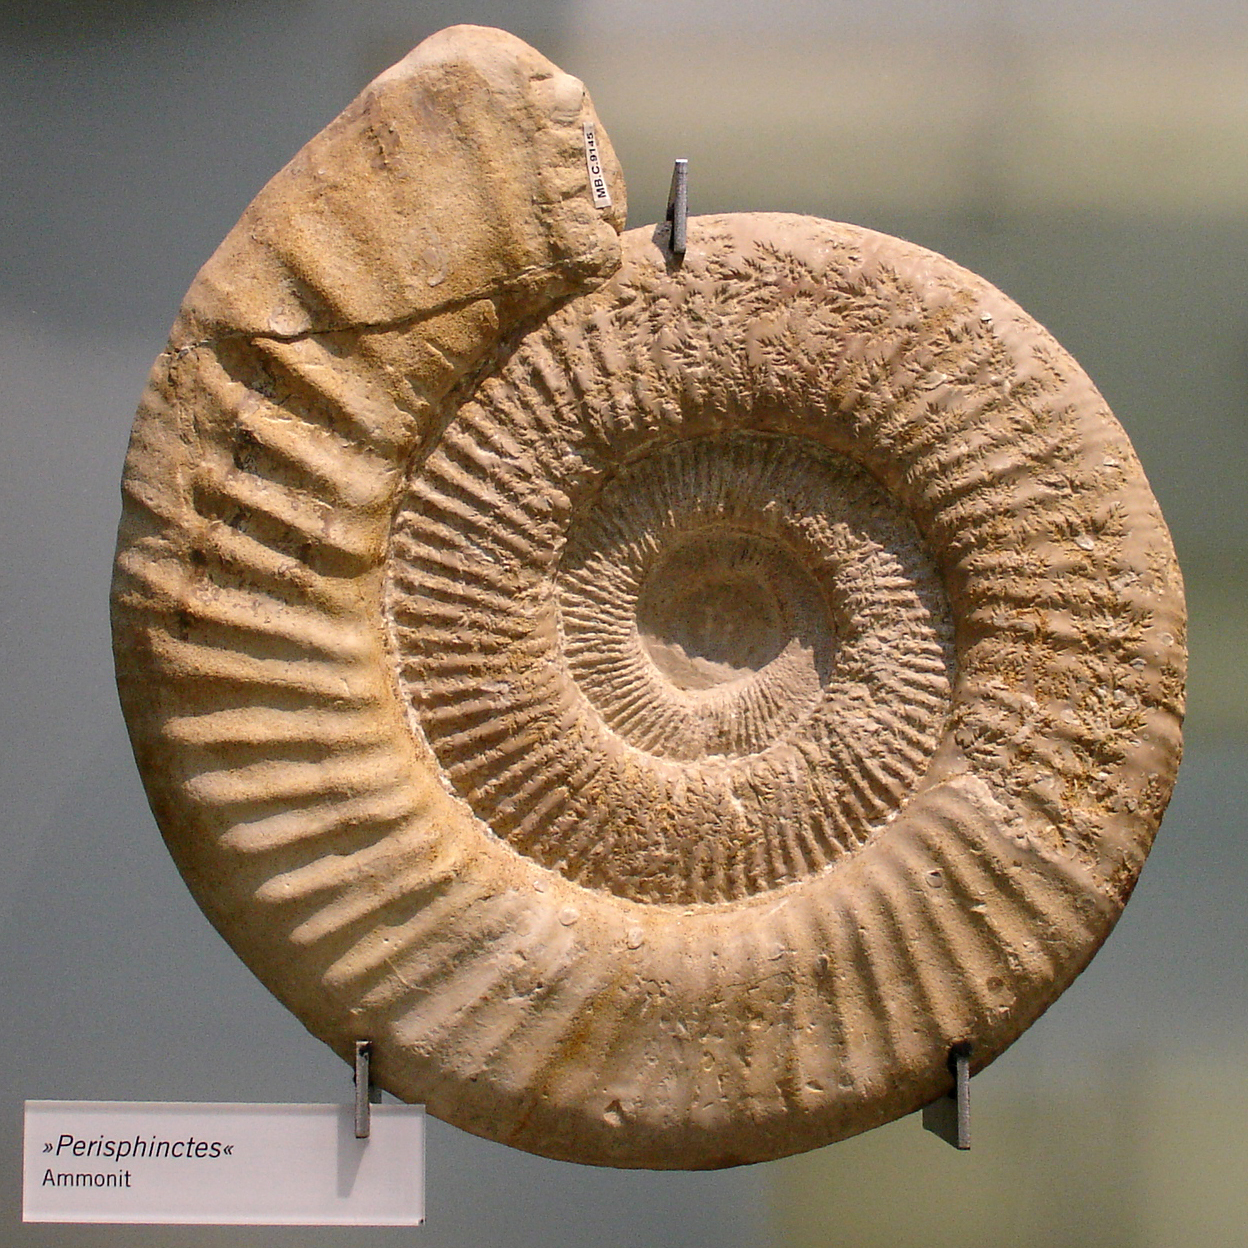
\includegraphics[scale=0.5]{img/ammonite.jpg}

And here is a map generated directely by shell commands in the SConstruct file. 

%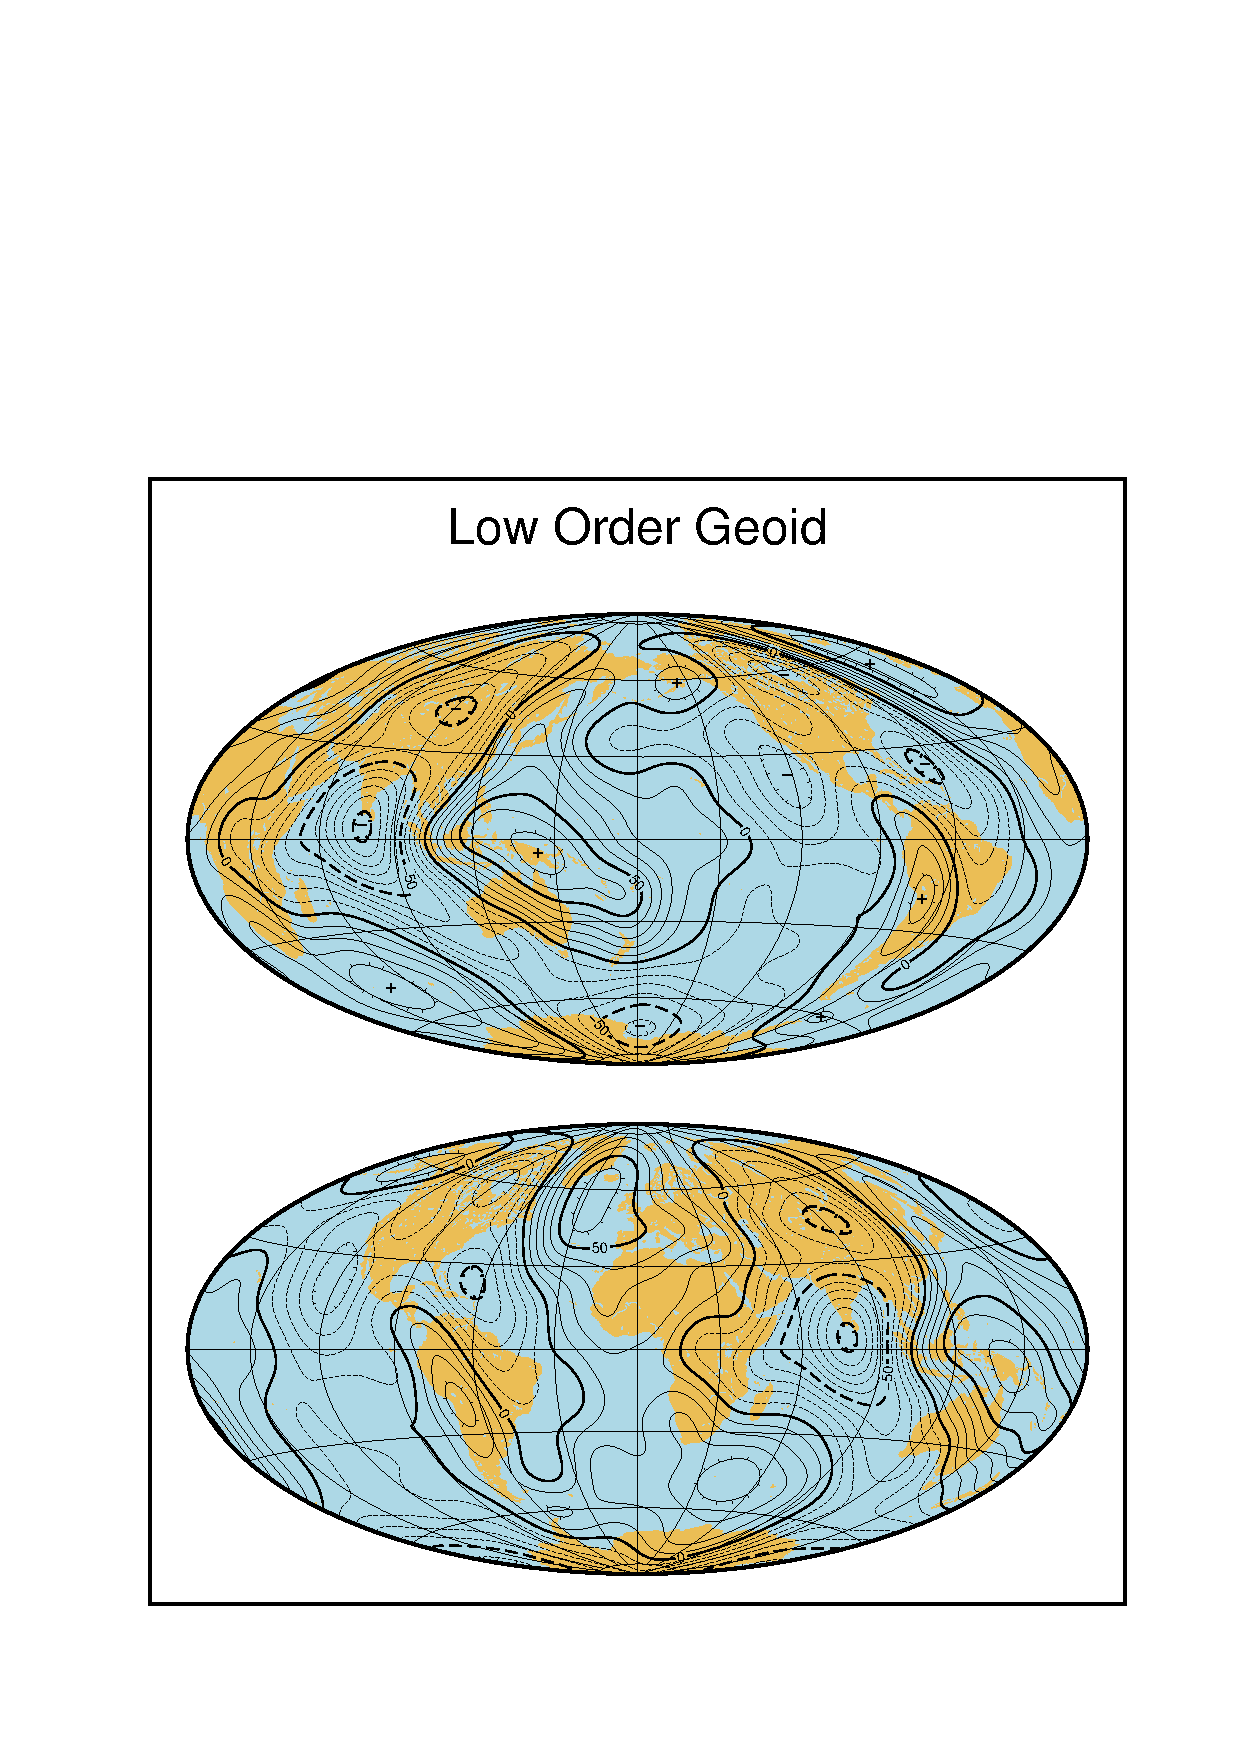
\includegraphics[scale=0.5]{fig/map1.pdf}

Here will be a tikZ illustration. 


\pagestyle{empty}
\pgfdeclarelayer{background}
\pgfdeclarelayer{foreground}
\pgfsetlayers{background,main,foreground}

\xdefinecolor{darkgreen}{RGB}{175, 193, 36}
\newcounter{cntShader}
\newcounter{cntRoot}
\setcounter{cntShader}{20}
\def\couleur{darkgreen}

\begin{tikzpicture}
    \foreach \y in {86,38,15}{
        \setcounter{cntShader}{1}
        \coordinate (a) at (0,0);
        \coordinate (b) at (0:1);
        \foreach \x in {1,...,\y}{%
            \coordinate (c) at ($ (b)!1cm!270:(a) $);
            \begin{pgfonlayer}{background}
                \draw[fill=\couleur!\thecntShader] (a)--(b)--(c)--cycle;
            \end{pgfonlayer}
            \setcounter{cntRoot}{\x}
            \addtocounter{cntRoot}{1}
            \node[fill=white,draw,circle,inner sep=1pt] at (c)
                {$\sqrt{\thecntRoot}$};
            \coordinate (b) at (c);
            \pgfmathsetcounter{cntShader}{\thecntShader+4}
            \setcounter{cntShader}{\thecntShader}
       }
    }
    \node[fill=white,draw,circle,inner sep=1pt] at (0:1) {$\sqrt{1}$};
\end{tikzpicture}


And biography. 

And maybe a madagascar exemple. 


\end{document}